\documentclass[a4paper,pra,aps,twocolumn,superscriptaddress,10pt,final]{revtex4-2}
\usepackage[pretty,uselistings]{revquantum}
% \usepackage[brazil]{babel}
\usepackage[T1]{fontenc}
\usepackage[utf8]{inputenc}
\usepackage{stmaryrd} 
\SetSymbolFont{stmry}{bold}{U}{stmry}{m}{n} 
\usepackage{bm}
\usepackage{amsmath}
\usepackage{amssymb}
\usepackage{amsfonts}
\usepackage{silence}
\WarningFilter{revtex4-2}{Repair the float}
\usepackage{anyfontsize}
\usepackage{lipsum}
\usepackage{float}
\usepackage{graphicx}
\usepackage{multirow}
% \usepackage{multicol}
\usepackage{wrapfig}
\usepackage[paperwidth=210mm,paperheight=297mm,centering,hmargin=2cm,vmargin=2.5cm]{geometry}
% \usepackage{physics}
\usepackage{siunitx}
%=============================================================================
% FRONT MATTER
%=============================================================================
% \graphicspath{{..imgs/}}

\begin{document}

\title{Atividade prática da disciplina de Circuitos Elétricos 1}

\author{Paulo Vinicius Pereira Pinheiro}
\email{paulovpp@gmail.com}
\affiliation{UNINTER - Centro Universitário Internacional}
\affiliation{RU: 3760288}
\affiliation{PAP: Juazeiro do Norte, CE. CEP: 63.000-000}

\date{\today}

\begin{abstract}
    A crescente necessidade por segurança nas transações online traz à tona um problema de grande complexidade: até quando os protocolos atuais de segurança da informação serão capazes de nos manter seguros? Inúmeros são casos de quebra de segurança ou vazamento de dados. Mesmo com uma grande quantidade de métodos utilizados para comunicação segura, não há garantias de plena segurança para nenhum deles. Dentre todos os métodos existentes, destaca-se a criptografia. De forma simétrica ou assimétrica, o ato de criptografar uma mensagem é torná-la inelegível a aqueles à quem a mensagem não se destina. A criptografia é um dos tópicos abordados na disciplina de matemática computacional do curso de engenharia da computação da UNINTER. E o trabalho realizado trata do assunto de forma aplicada. Através da Cifra de Feistel, pode-se compreender com mais clareza os procedimentos de codificação e decodificação de mensagens criptografados. Pra tal, são solicitados os seguintes procedimentos: que sejam codificados os 4 primeiros caracteres do primeiro nome do aluno utilizando-se a cifra simétrica de Feistel com apenas 2 estágios, utilizando o último dígito do RU não nulo, $K$,  como a chave criptográfica para ambos os estágios. Deve-se utilizar também como função $F$ um shift left, cíclico, de $K$ posições. Solicita-se também que a mensagem codificada seja preparada para transmissão e que, em seguida, haja o processo de decodificação, comprovando assim a reciprocidade do processo.
    
    
\end{abstract}

\maketitle

%=============================================================================
% MAIN DOCUMENT
%=============================================================================

\section{Introdução}
\label{sec:intro}

    Criptografia é o processo de codificar ou embaralhar uma mensagem que se deseja transmitir, de tal modo que apenas aquele à quem a mensagem se destine tenha meios para identificar seu conteúdo. Inúmeros são os usos da criptografia para comunicação segura, como em transações financeiras, governamentais e empresariais. 

    % \begin{figure}[!htpb]
    %     \centering
    %     \label{fig:cifra}
    %     \caption{Cifra de Feistel.}
    %     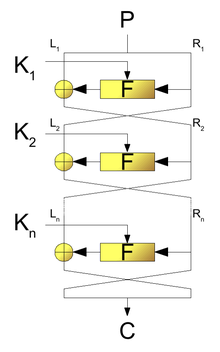
\includegraphics[width=0.25\textwidth]{feistel.png}
    %     \begin{center}
    %         \scriptsize{Fonte: \url{https://pt.alegsaonline.com/art/33900}}
    %     \end{center}
    % \end{figure}

    Os processos de codificação e decodificação são idênticos. Eles consistem em dividir a mensagem em dois blocos de tamanhos iguais, aplicar ao segundo bloco uma função \textit{HASH} $F$ de embaralhamento e após, com o primeiro bloco, realizar uma função XOR. A função \textit{HASH}  é gerada a partir de um valor aleatório, conhecido como a chave do processo. Após a função XOR, o resultado é concatenado ao segundo bloco utilizado antes da aplicação da função $F$, que toma a posição inicial no bloco em formação.

    A operação de decodificação acontece da mesma forma. As chaves utilizadas nas iterações de decodificação precisam ser as mesmas utilizadas no processo de codificação. Daí decorre sua classificação de cifra de chave simétrica. Portanto, nasce aí o maior problema da cifra de chave simétrica: como compartilhar a chave?
    
    O desenvolvimento deste trabalho, esclarecido na seção~ a seguir, está dividido em duas partes: a subseção trata da codificação e a subseção trata da decodificação. Conclusões e considerações finais encontram-se na seção.




\section{Procedimento experimental}
\label{sec:proced_exp}

    A presente seção tem por objetivo apresentar os procedimentos realizados na atividade em questão. Destaca-se que como a atividade é bastante extensa, a seção foi subdividida em quatro partes, correspondendo cada uma a uma questão proposta.

    \subsection{Experimento 1: Lei de Ohm}
    \label{subsec:exp1}

    Neste primeiro experimento, foi solicitada a montagem real do circuito apresentado na figura~\ref{fig:circuito1} e sua simulação utilizando um circuito digital. O circuito é composto apenas pela fonte de tensão contínua e um resistor com o valor deduzido do RU do aluno. No caso do autor deste trabalho, com o RU de número 3760288, o valor do resistor é de $\qty{880}{\ohm}$. Como não há um resistor deste valor, foram utilizados dois resistores em uma associação em série, com os valores iguais a $\qty{560}{\ohm}$ e $\qty{330}{\ohm}$, o que resulta na resistência equivalente igual a $\qty{890}{\ohm}$

    \begin{figure}[htpb]
        \centering
        \label{fig:circuito1}
        \caption{Circuito do Experimento 1}
        \includegraphics[width=0.4\textwidth]{imgs/fig1.png}\\
        \scriptsize{Fonte: Elaboração própria.}
    \end{figure}
   
    suficientes para proceder com a codificação. Para o segundo \textit{nibble} de cada caractere é executada a função $F$ do tipo \textit{shift left} cíclica oito($8$) vezes, e na sequência o resultado é submetido a uma função $XOR (\oplus)$ com o primeiro nibble. Na tabela elucida-se os resultados obtidos para cada caractere:

    \begin{figure}[htpb]
        \centering
        \label{fig:circuito2}
        \caption{Circuito do Experimento}
        \includegraphics[width=0.4\textwidth]{imgs/fig2.png}\\
        \scriptsize{Fonte: Elaboração própria.}
    \end{figure}

    Para formação da sequência de caracteres codificada, são utilizados dois \textit{nibbles} para cada caractere: o primeiro é obtido do \textit{nibble} prévio à codificação, e o segundo será o resultado da função XOR aplicada, ambos contidos nas colunas 3 e 4 da tabela. Aplicando a concatenação para todos os caracteres, obtêm-se então a mensagem codificada após uma iteração:

    A sequência de caracteres codificada após a segunda iteração é dada pela tabela. Essa será a mensagem CODIFICADA que deverá ser transmitida para um destinatário.

    % \begin{table}[!htpb]
    %     \caption{Mensagem codificada após duas iterações.}
    %     \label{tab:tab5-mens}
    %     \begin{tabular}{|c|}
    %     \hline
    %     \textbf{Mensagem codificada}  \\ \hline
    %     0101 0101 0110 0111 0111 0010 0110 1010     \\ \hline
    %     \textbf{V $\qquad\quad$ g $\qquad \quad$ r $\qquad \quad$ j} \\ \hline
    %     \end{tabular}%
    % \end{table}

    A  amostra a sequência de caracteres codificada após a segunda iteração, realizando assim a codificação solicitada. Na sequência, o processo de decodificação é desenvolvido.
programming 
\section{Análise e Resultados}
\label{sec:analise_resultados}

    Como prova de conceito, realiza-se agora o processo de decodificação da mensagem previamente codificada. O processo decorre de forma semelhante à codificação, através da aplicação sequenciada das funções $F$ e XOR.
    
    Seguindo o mesmo procedimento da codificação, na primeira iteração da decodificação, o segundo nibble de cada caractere é submetido à função $F$ e em seguida, com o primeiro nibble, a função XOR. Aplicando-se as funções para todos os caracteres, com seus resultados mostrados na tabela~\ref{tab:tab6-funcao}, obtêm-se a sequência de caracteres decodificada mostrada na tabela~\ref{tab:tab7-iter1-deco}.

    \begin{table}[!htpb]
        \caption{Funções $F$ e XOR para $1^a$ iteração da decodificação.}
        \label{tab:tab6-funcao}
        \begin{tabular}{|cc|c|c|}
            \hline
            \multicolumn{2}{|c|}{\textbf{Mensagem}} & \textbf{Função $F$} & \textbf{XOR ($\oplus$)} \\ \hline
            \multicolumn{1}{|c|}{0101}    & 0101    & 0101                & 0000                                 \\ \hline
            \multicolumn{1}{|c|}{0110}    & 0111    & 0111                & 0001                                 \\ \hline
            \multicolumn{1}{|c|}{0111}    & 0010    & 0010                & 0101                                 \\ \hline
            \multicolumn{1}{|c|}{0110}    & 1010    & 1010                & 1100                                 \\ \hline
        \end{tabular}
    \end{table}
    
    \vspace{-0.5cm}
    
    \begin{table}[!htpb]
        \caption{Mensagem decodificada com apenas uma iteração.}
        \label{tab:tab7-iter1-deco}
        \begin{tabular}{|clll|}
        \hline
        \multicolumn{4}{|c|}{\textbf{Mensagem codificada}}            \\ \hline
        \multicolumn{4}{|c|}{0101 0000 0111 0001 0010 0101 1010 1100} \\ \hline
        \end{tabular}%
    \end{table}

    A segunda iteração da decodificação ocorre de forma semelhante a primeira mas sem a inversão dos nibbles ao final da formação dos caracteres. A tabela~\ref{tab:tab8-funcao-deco} mostra os resultados das aplicações das funções $F$ e XOR para cada caractere da segunda iteração:
    
    \vspace{-0.25cm}

    \begin{table}[!htpb]
        \caption{Funções $F$ e XOR para $2^a$ iteração da decodificação.}
        \label{tab:tab8-funcao-deco}
        \begin{tabular}{|cc|c|c|}
            \hline
            \multicolumn{2}{|c|}{\textbf{Mensagem}} & \textbf{Função $F$} & \textbf{XOR (\textbackslash{}oplus)} \\ \hline
            \multicolumn{1}{|c|}{0101}    & 0000    & 0101                & 0101                                 \\ \hline
            \multicolumn{1}{|c|}{0110}    & 0001    & 0111                & 0110                                 \\ \hline
            \multicolumn{1}{|c|}{0111}    & 0101    & 0010                & 0111                                 \\ \hline
            \multicolumn{1}{|c|}{0110}    & 1100    & 1100                & 0110                                 \\ \hline
            \end{tabular}
    \end{table}

    A formação do byte correspondente a cada caractere é realizada sem a inversão dos nibbles ao final das operações. A tabela~\ref{tab:tab9-mens-deco} mostra os resultados das concatenações utilizadas para composição dos caracteres da mensagem final decodificada.

    \begin{table}[!htpb]
        \caption{Mensagem decodificada.}
        \label{tab:tab9-mens-deco}
        \begin{tabular}{|c|}
            \hline
            \textbf{Mensagem codificada}                      \\ \hline
            0101 0000 0110 0001 0111 0101 0110 1100           \\ \hline
            \textbf{P $\qquad \quad \quad$ a $\quad \qquad$ u $\qquad \quad \quad$ l} \\ \hline
        \end{tabular}%
    \end{table}

\section{Conclusão}
\label{sec:conclusion}
    
    Neste trabalho foram realizadas a codificação e decodificação de uma mensagem pela Cifra de Feister, um modelo de criptografia de chave simétrica e de bloco geralmente utilizada com 64 bits. A mensagem original foi determinada a partir dos primeiros quatro caracteres do primeiro nome do autor. A função $F$ solicitada como foi a \textit{shift left} cíclico pelo número de vezes correspondente ao último dígito não inteiro do RU. E o número de interações solicitado para cada processo foi de duas iterações com a mesma chave cada.
    
    A seção de desenvolvimento foi dividida em duas partes, para os processos de codificação e decodificação correspondentemente. Tabelas foram apresentadas com o passos intermediários e os resultados preliminares das operações. As mensagens codificada e decodificada podem ser encontradas correspondentemente nas tabelas Os resultados estão de acordo com o solicitado no enunciado do trabalho.

    Conclui-se também que a Cifra de César possui um baixo custo de processamento para codificação e decodificação, já que é realizada em bloco. Porém, como trata-se de uma cifra simétrica, o problema de  compartilhamento da chave ainda permanece. Espera-se que o problema de compartilhamento de chaves privadas possa ser resolvido na computação clássica como já é trabalhado na computação quântica.

    \vspace{-0.5cm}

    \begin{acknowledgments}
        O autor agradece aos professores, tutores e a todo pessoal responsável pela disciplina de matemática computacional pela oportunidade de produzir tal trabalho que sem dúvida, aprofundou o conhecimento adquirido no período de estudos.    

        Trabalho realizado em \LaTeX.
    \end{acknowledgments}
% \bibliography{example}

%=============================================================================
% APPENDICES
%=============================================================================

\appendix

% %=============================================================================
\section{Processo de codificação}
\label{apx:code}

    Abaixo segue uma imagem do processo de codificação e decodificação da mensagem solicitada usando a Cifra de Feister.

\onecolumngrid

    % \begin{figure*}[!htpb]
    %     \centering
    %     \caption{Imagem retirada do microsoft excel com o processamento da cifra solicitada.}
    %     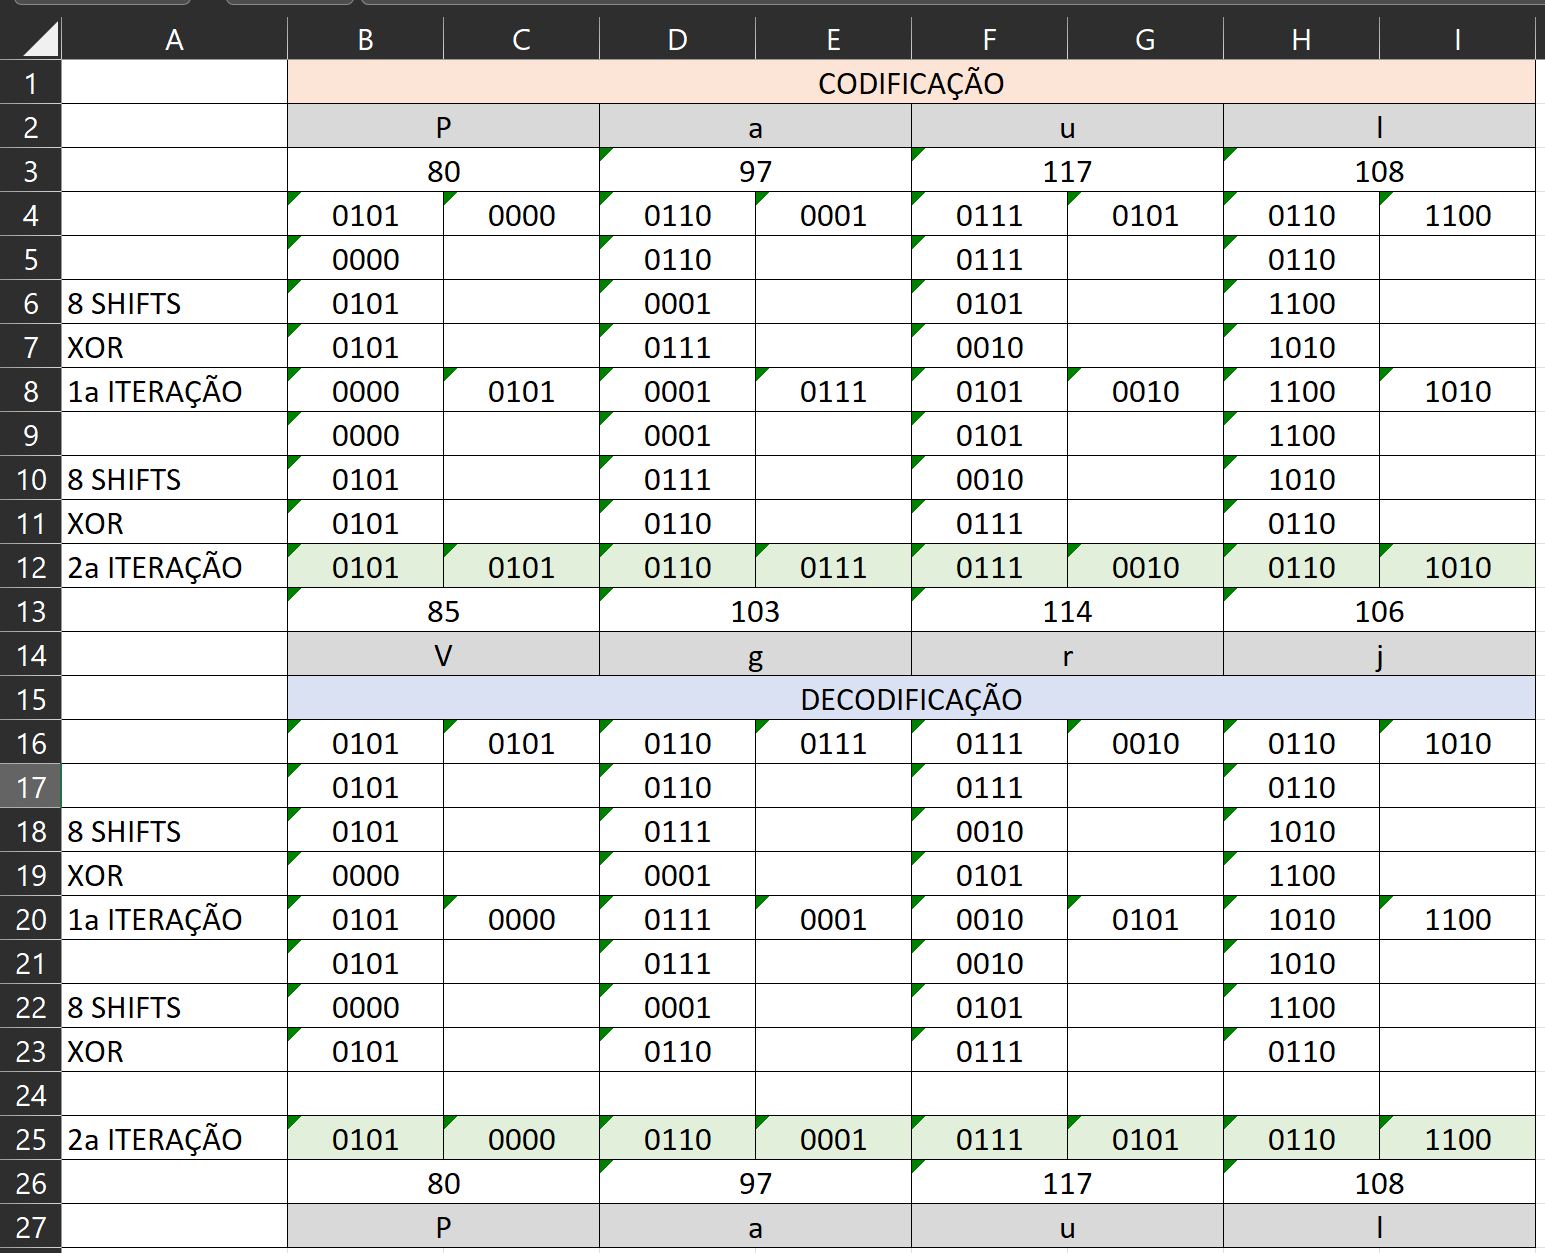
\includegraphics[width=\textwidth]{Tabela-cifra.png}
    %     \label{fig:Tabela-cifra}
    % \end{figure*}

\end{document} 